\section{Framework Overview}
\label{sec:system}

\begin{figure}[th]
\centering
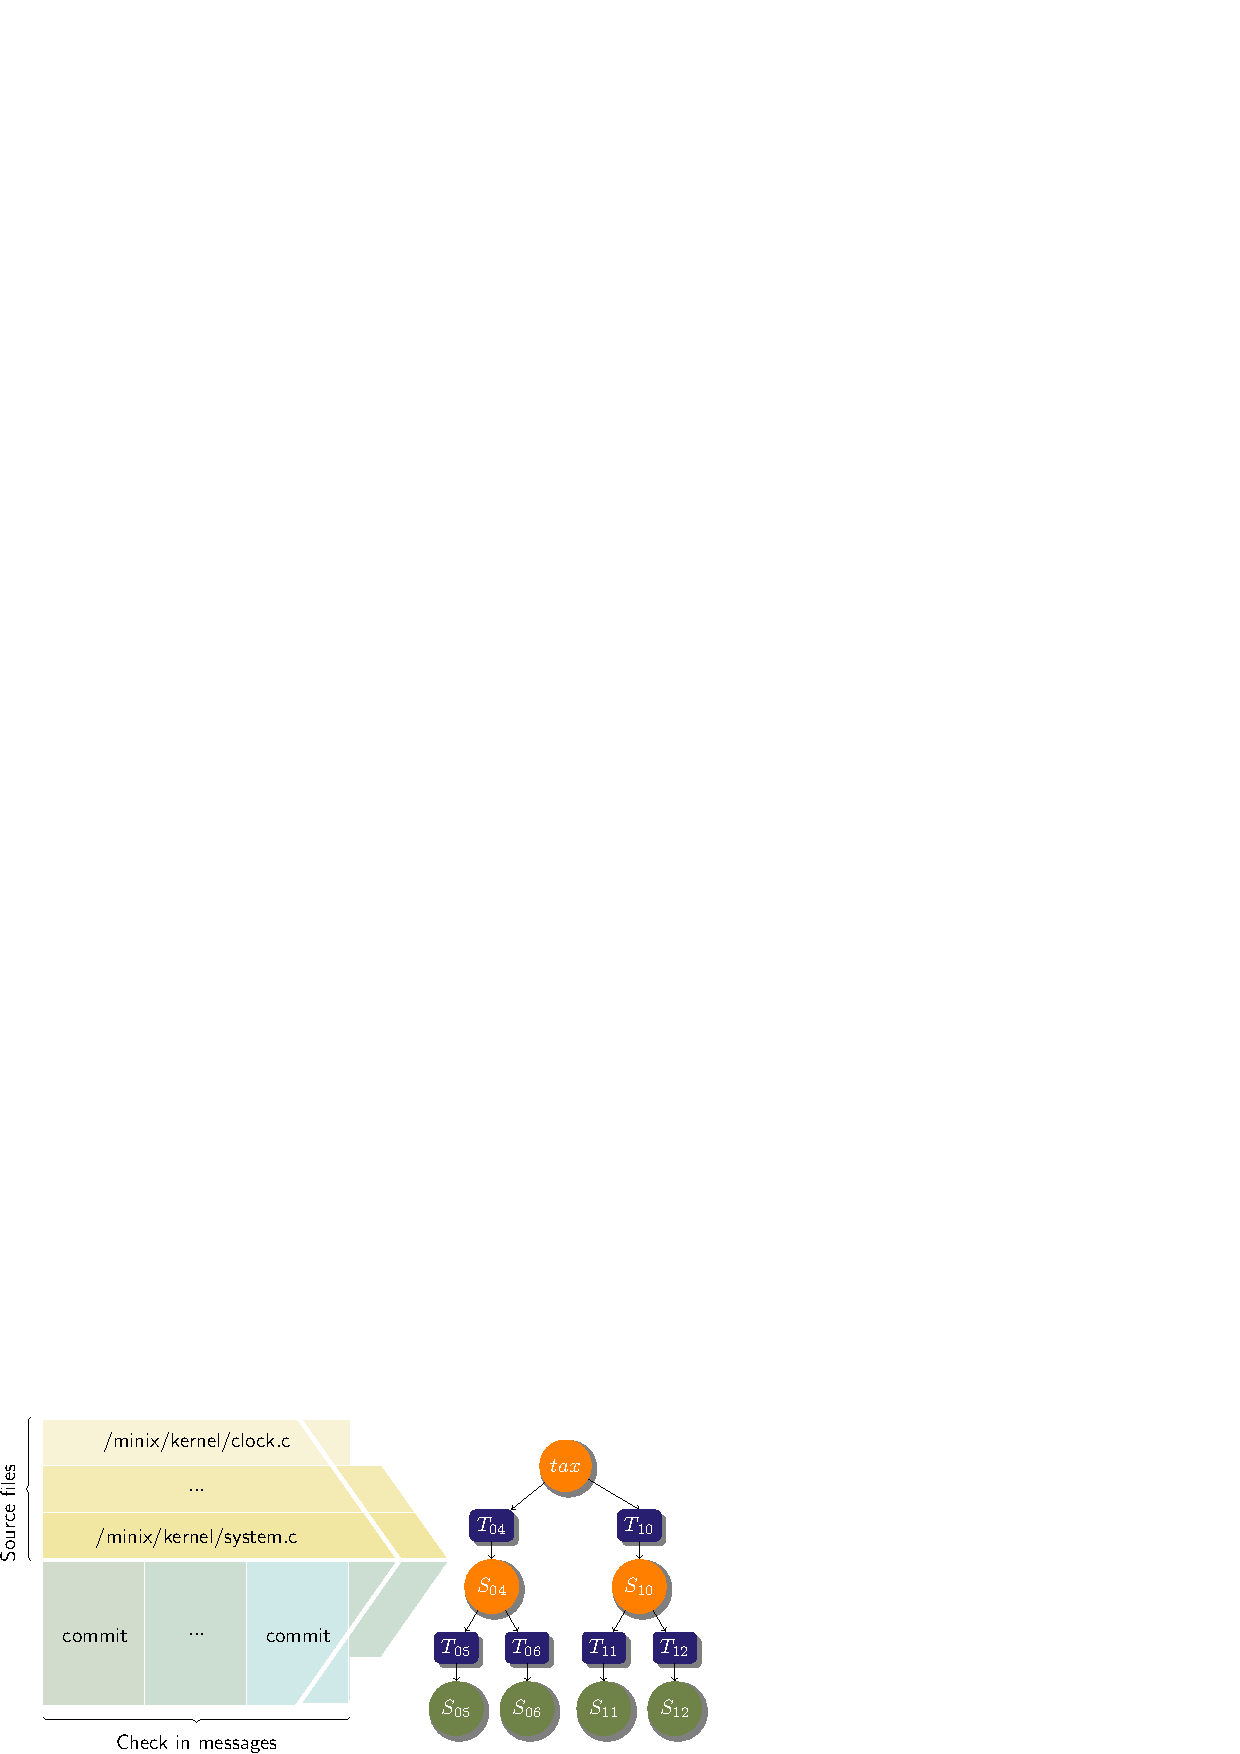
\includegraphics[width=1.0\columnwidth]{picture/framework.jpg}
\caption{ICQ Workflow}
\label{fig:framework}
\end{figure}

The overview of ICQ framework is illustrated in in~\figref{fig:framework}.
ICQ can be broken down into the following phases: feature definition, 
dataset filtering and evaluation, and model evaluation. With ICQ, we 
discover whether the data have spurious cues, and whether a model is 
sensitive to a particular linguistic feature during inference.

%WeWe evaluate the information leak in the datasets by statistical cues only. 
%First, we formulate  a number of NL reasoning tasks in a general form. 
%Then based on the cues associated with each label, 
%we design a number of metrics to measure the correlation between words
%and labels. Such correlation scores are called ``cue scores'' because they are 
%indicative of potential cue patterns. Afterwards, we aggregate the scores using a number of simple statistical
%models to make the predictions. Finally, we show how to split a dataset into
%the easy and hard parts using the above fast predictions.

\subsection{Linguistic Features}
\label{sec:extract}

In this work, we have considered the following list of linguistic features: 
Word (unigram word in the task), 
Typos, NER (appropriately understanding named entities), 
Tense (understanding temporal order of events), Negation, 
Sentiment, and Overlap (overlapping words between premise and hypothesis). 
This list is by no means exhaustive, but just a starting point for users, 
who can come up with additional features that are specific 
to their task or domain. We use $F$ to denote the feature set.

\subsubsection{Word} For a dataset $X$, 
we collect a set of all words $\mathcal{N}$ that exist in $X$. 
%These 
%words can be word or cross-word that consists of a pair of
%unigrams, one from the premise and other from the hypothesis.
%the token pair between $p$ and $h$.
The feature metric for a word measures the disparity of the word's appearance under 
 a specific label. 
%The cross-unigrams, such as  ``swimmer-sea'' in~\exref{exp:snli}, 
%represent the 
%relational unigrams in a dataset. 
%The ``swimmer-sea'' cross-unigram can be identified as a cue if it always appear in the instances with 
%one label, like entailment.

Let $w$ be a word in $\mathcal{N}$, we compute a scalar statistic metric 
called {\em cue score}, $f^l$, for a label $l$. 
We use conditional probability(CP)
as the feature score to measure the correlation between words and labels: 
\begin{equation}
    cp^{(w,l)} = \frac{\#(w, l)}{\#(w)}
\end{equation}

We rank the words by feature score to $N^{'}$ and 
only treat top $k$ words as features:

\begin{equation}
    F_{W_i} = {w}_{i} , i \in 1...k \wedge w_{i} \in N^{'}.
\end{equation} 

We further define accuracy deviation score ($\mathcal{D}$)
\begin{equation}
    \mathcal{D} = {Acc} - {Majority},
\end{equation}
where $Acc$ is the prediction accuracy of a simple logistic regression
model trained on the CP feature of all words or of a hypothesis-only
model, and $Majority$ is the accuracy of vote by majority.
As \figref{fig:d_figure} shows, accuracy of the linear model using 
the CP features is very similar to the more complex hypothesis-only models 
(Pearson score of 97.17\% for fastText and 97.34\% for Bert), 
which indicates CP is a good choice of word feature.

\begin{figure}[th]
\centering
\includegraphics[width=0.7\columnwidth]{picture/d_figure.pdf}
\caption{Deviation scores for three prediction models on all 12 datasets. 
``Our'' means our logistic regression model.}
\label{fig:d_figure}
\end{figure}

%of $w$ with respect to label $l$ as
%%\KZ{Consider changing $\mathcal{F}$ to $\mathcal{B}$ to avoid confusion with $f$?}
%
%\begin{equation}
%    f_{\mathcal{F}}^{l} = f_{\mathcal{F}}(w, l),    
%\end{equation}
%%We call $f_{\mathcal{F}}^{(k,l)}$ \textit{cue metric}, 
%where $f_{\mathcal{F}}^{l}$ is a function which measures how much spurious information can be conveyed by token $w_k$ for a particular label $l$. 
%$\mathcal{F}$ is a set of cue metrics that we used for computing the \textit{cue score}. 

\subsubsection{Sentiment}

We assign sentiment features $F_{S}$ as 
positive, negative, or neutral to each hypothesis $h$: 
$S(h) = \sgn(\mbox{num of positive words} - \mbox{num of negative words})$.
%in the hypothesis.
The sentiment polarity of a word
is determined by a look-up from pre-trained
sentiment lexica\footnote{NLTK: \url{https://www.nltk.org}}. 

\subsubsection{Tense}

Considering that the temporal order of events can be also 
important information for inference tasks, we include 
\textit{past}, \textit{present}, \textit{future} as Tense features $F_{Tense}$. 
The tense is determined by verb tags.
\subsubsection{Negation}

Much work has observed that strongly negative words (``no'', ``not'') 
cause the model to predict contradiction for
neutral or entailed statements. Thus we think negation feature 
$F_{Neg}$ can be a factor which affects models in decision-making. 
Negation is decided with dependency parsing tags~\footnote{Scipy: \url{https://www.scipy.org}}.

\subsubsection{Overlap}
In many cases, substantial word-overlap between the premise and the
hypothesis sentences causes wrong entailment prediction, 
even if they are unrelated. 
%Very little word overlap causes a prediction
%of neutral instead of entailment. 
Thus we wonder 
whether overlap feature $F_{O}$ really influences models.

\subsubsection{NER}
The failure for the NER tests in CheckList
indicates that these models are relying on shortcuts.
%For example anchoring on named entities too strongly
%instead of understanding named entities and their
%impact on whether questions are duplicates. 
We also take in NER feature $F_{NER}$, like \textit{Location}, in our feature test.

\subsubsection{Typos}
The premise or the hypothesis is ill-formed because of spelling errors. 
Typo feature $F_{Typos}$ may also be learned by models as off-site information. 
We use a pretrained spelling model~\footnote{\url{https://github.com/barrust/pyspellchecker}} 
to get the typo information in a sentence. 

%We only pay attention to the features which have enough test data for model evaluation.
%In addition, we can analysis the credibility of test data through 
%the Kullback-Leibler (KL) Divergence. If a train dataset distribution is unbalance, 
%a similar distribution between train and T
%test can lead to insufficient test which test the cues mostly with a certain label. 

\subsection{Data Set Filter and Evaluation}
\label{sec:generate}
%Given the features $F$, 
We can filter cases with specific features $F$ from the training and test data. 
In~\figref{fig:framework}, the blue 
distribution and red distribution represent  the training and test data 
distribution on the predication values respectively. 
We use mean square error (MSE) to measure the balance 
of a feature in a dataset. If the filtered training data distribution is 
unbalanced on a feature, this feature can be seen as bias.  
If this bias also exists in test data, indicating 
a similar distribution exists in the test data, 
this feature is considered a cue. 

Dotted arrows in \figref{fig:framework} indicate the visualization of 
the distributions.
We show the distribution of some filtered SNLI datasets 
in~\figref{fig:dataset_result}. 
We can see that Word feature ``speaking'' mostly correlates with 
label ``entailment''. So ``speaking'' is a bias. 
The similar shape between the training and test data distribution indicates 
this bias is a cue. Low Jensen-Shannon Divergence (JSD) score between the two
distributions re-affirms our conclusion. 
Compared with ``speaking'', Word feature ``pushing'' has lower MSE 
score, but is still much higher than average distribution.  
Thus ``pushing'' is also a bias. However we can observe that there is little similarity between 
the train and test distribution. Therefore ``pushing'' is not a cue.
%With filtering and visualizing, we can analysis the biases 
%and cues in datasets. 
%Biases can influence models and cues make the evaluation unauthentic. 

\begin{figure}[th]
\centering
\includegraphics[width=1.0\columnwidth]{picture/dataset_result.jpg}
\caption{Two examples of dataset distribution on features.}
\label{fig:dataset_result}
\end{figure}

\subsection{Model Evaluation}
\label{sec:model}

Similar to discovering biases and cues, we can probe models by  
comparing the distribution of the model prediction results and 
the training data.
%but don't provide new method for data augmentation. 
%We require a more fair dataset to test if a model is sensitive to a feature. 
The filtered test dataset of a feature in \figref{fig:framework} (red) is unbalanced among 
labels. The number of cases for each label can be denoted as $c_{ent}, c_{neu}, c_{con}$~(in 
SNLI task). If any of these number is smaller than a threshold $\sigma$, 
we won't consider to test this feature, because
 this feature is not well supported by enough data. 
%If the smallest number of samples among different labels is lower than 
%a threshold $\sigma$, we won't consider to test this feature. Because
% this feature is not well supported by enough data. 
The smallest number can be denoted as $c_{min}=min(c_{ent}, c_{neu}, c_{con})$.
To make the result more intuitive and fair, 
we flatten the distribution by removing $c_{l} - c_{min}$ cases from the filtered cases with label $l$ 
resulting in the orange ``stress test'' 
in \figref{fig:framework}. 
Then we test the model on this stress test. 
The similarity between prediction result (green) and 
training data distribution (blue) on a feature indicates how the model 
is influenced by the appearance of this feature in training data. 
For example, in \figref{fig:model_result}, we use 
ESIM~\cite{chen2016enhanced} model on SNLI. 
We can find that the model is affected by some bias features. 
Given ``pushing'', it still prefers to choose \textit{contradiction}. 
Further, it prefers to choose \textit{entailment} or \textit{neutral} with ``speaking''.  
JSD score for these two examples are also very low. 
%With comparison, we can find that models are sensitive to some bias features. 

%It is insufficient for testing if the filtered test data size is quite small or samples on 
%some label is rare which bellow a threshold $\sigma$. 
%Thought we can't generate cases for feature, we can point out what kind of 
%test samples should be augmented. 

\begin{figure}[th]
\centering
\includegraphics[width=1.0\columnwidth]{picture/model_result.jpg}
\caption{Two examples of model prediction result distribution on features.}
\label{fig:model_result}
\end{figure}


%The similarity is 
%calculated by Kullback-Leibler (KL) Divergence.
